%%
%% ju_liu_presentation.tex
%% 
%% Made by ju
%% Login   <ju@ubuntu>
%% 
%% Started on  Tue Aug 25 13:37:40 2009 ju
%% Last update Tue Aug 25 13:37:40 2009 ju
%%

\documentclass{beamer}

\usepackage{beamerthemesplit}
\usepackage[english]{babel}
\usepackage[latin1]{inputenc}
\setbeamercovered{transparent}

\title{GMPLS multi-layer path computation}
\author{Ju Liu -- Acreo AB}
\date{\today}

\begin{document}

\frame{\titlepage}

\section[Outline]{}
\frame{\tableofcontents}

\section{Introduction}
\subsection{Overview of the problem}
\frame
{
  \frametitle{What is the problem?}

  \begin{itemize}
  \item<1-> One billion Internet users.
  \item<2-> A lot of services are requested, like P2P, IPTV and VoIP.
  \item<3-> The network resources of the Internet Service Providers
    are under heavy stress.
  \end{itemize}
}
\frame
{
  \frametitle{What are the demands?}

  The ISPs need to:  
  \begin{itemize}
  \item<1-> Control the traffic flows and react dynamically to the
    changes in the network topology.
  \item<2-> Enable reliable automatic service provisioning throughout
    the entire network.
  \item<3-> Ensure a suitable Quality of Service for each type of
    service.
  \item<4-> \textbf{Traffic Engineering}.
  \end{itemize}
}
\subsection{Traffic Engineering}
\frame
{
  \frametitle{Traffic Engineering}

  Explicit routes:
  \begin{itemize}
  \item Traffic sharing and load balancing.
  \item Backup paths and error recovery mechanisms.
  \end{itemize}

  \begin{figure}[!hbp]
    \centering
    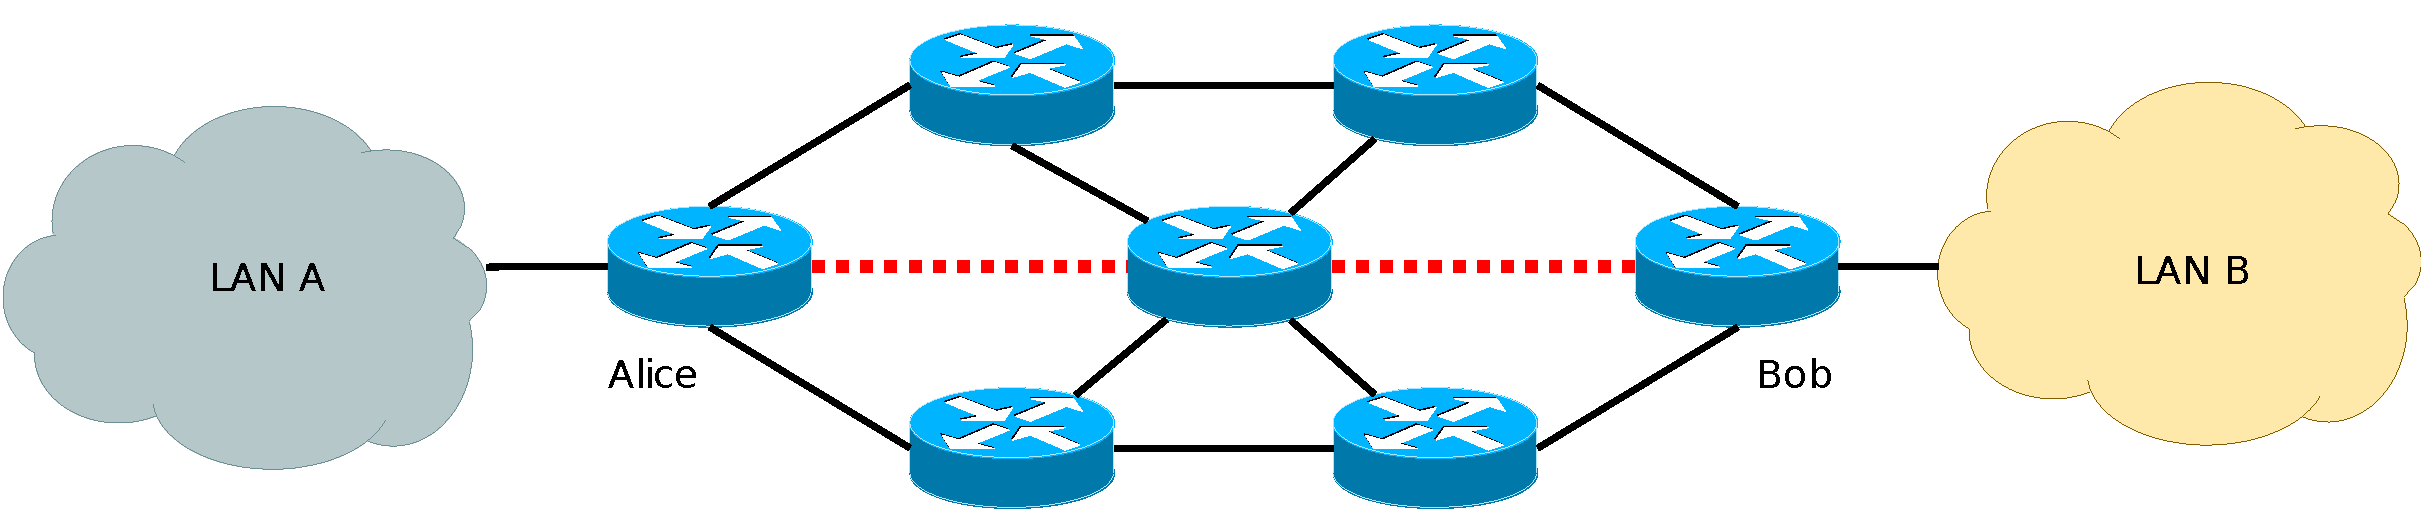
\includegraphics[width=1\textwidth]{img/mpls_te}
  \end{figure}
}
\frame
{
  \frametitle{Traffic Engineering}

  Constraint based routing:
  \begin{itemize}
  \item The shortest path is not always the best.
  \item Multiple constraints have to be considered at the same time.
  \item Different services may need different constraints.
  \end{itemize}

  \begin{figure}[!hbp]
    \centering
    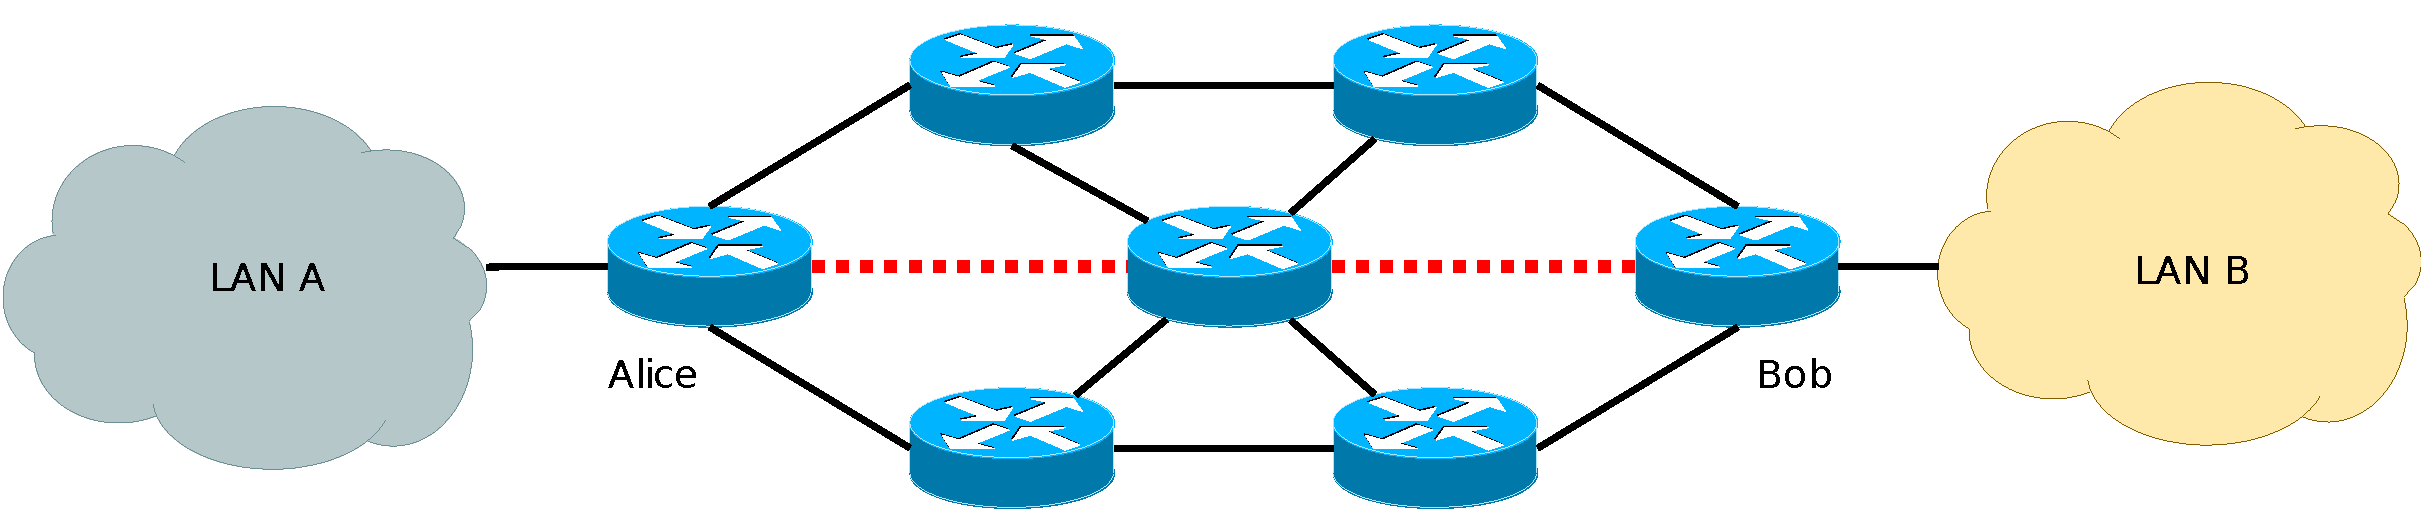
\includegraphics[width=1\textwidth]{img/mpls_te}
  \end{figure}
}

\section{MPLS and GMPLS}
\subsection{MPLS concepts}
\frame
{
  \frametitle{MPLS}
  
  \begin{itemize}
  \item<1-> \textbf{MPLS} stands for Multi-Protocol Label Switching.
  \item<2-> Introduced by the IETF to solve the problem of IP routing,
    which is based on addresses and longest prefix match.
  \item<3-> MPLS routing process is instead based on a \textit{small,
      fixed format label that identifies the packet to the network
      nodes}.
  \item<4-> An MPLS router is called Label Switching Router (LSR),
    while the path within the MPLS network is called Label Switched
    Path (LSP).
  \end{itemize}
}
\frame
{
  \frametitle{Label switching}

  \begin{itemize}
  \item<1-> A labeled packet enters in the LSR from one interface.
  \item<2-> Depending from the label and from the incoming interface, a new
    label and an outgoing interface are chosen.
  \item<3-> The label is swapped and the packet forwarded.
  \end{itemize}
  
  \begin{figure}[!hbp]
    \centering
    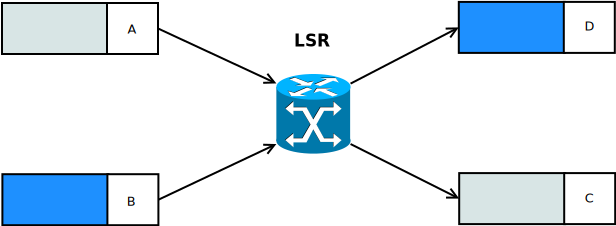
\includegraphics[width=0.7\textwidth]{img/label_switching}
  \end{figure}
}
\frame
{
  \frametitle{MPLS network}

  \begin{itemize}
  \item<1-> When the packet enters in the MPLS network, the IP
    destination address is analyzed and a label is assigned.
  \item<2-> From that moment, the packet is forwarded following the
    labels logic.
  \item<3-> When the packet exits from the MPLS network, the last
    label is analyzed and the packet is forwarded to the IP
    destination.
  \end{itemize}
  
  \begin{figure}[!hbp]
    \centering
    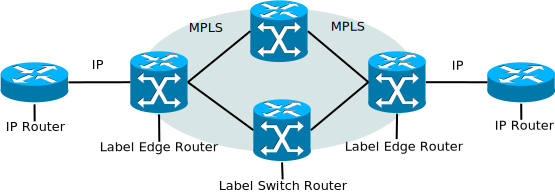
\includegraphics[width=0.8\textwidth]{img/mpls_net}
  \end{figure}
}

\subsection{GMPLS concepts}
\frame
{
  \frametitle{GMPLS definition}

  Generalized Multi-Protocol Label Switching (\textbf{GMPLS}) is suite
  of protocols designed to extend the concept of label switching to
  various transport network technologies.
}
\frame
{
  \frametitle{Control and data plane}

  \begin{itemize}
  \item<1->The great innovation brought in by GMPLS is the complete
    separation of the control plane and the data plane: the former is
    used to control the setup of end-to-end connections, while the
    latter is used to actually transfer the data.
  \item<2-> While the control plane is common to every different
    technology and remains IP-based, the data plane can now diversify
    and support multiple types of switching: packets, frames,
    time-slots, wavelengths and fibers can be present at the same time
    in a GMPLS network.
\end{itemize}
}
\frame
{
  \frametitle{Switching capabilities}

  Therefore, a GMPLS network device can be:
  \begin{itemize}
    \item \textit{Packet Switch Capable} (PSC):\\
      Router/ATM Switch/Frame Reply Switch
    \item \textit{Time Division Multiplexing Capable} (TDMC):\\
      SONET/SDH ADM/Digital Cross-Connect
    \item \textit{Lambda Switch Capable} (LSC):\\
      Optical ADM/Optical Cross-Connect
    \item \textit{Fiber Switch Capable} (FSC)
  \end{itemize}
}
\frame
{
  \frametitle{A different label}

  \begin{itemize}
  \item<1-> In MPLS, there is no relation between the label and the packet to
    which it is associated.
  \item<2-> Instead, in GMPLS the label indicates a precise physical
    resource.
  \item<3-> The label in GMPLS must be therefore analyzed carefully.
\end{itemize}
}
\frame
{
  \frametitle{GMPLS tunneling}
  
  \begin{itemize}
  \item<1-> In MPLS, it is possible to tunnel an LSP inside another
    LSP by adding an additional label to the packet; the set of labels
    associated to a packet is called \textit{label stack}. Only the
    topmost label is considered during the routing process.
  \item<2-> In GMPLS, some technologies involved do not support
    stacking: for example, you can't encapsulate a wavelength inside
    another one and extract it at the end of the tunnel.
  \item<3-> The hierarchy of the tunnels has to be based on the
    natural difference in granularity of the different network
    technologies: packets are nested in a time-slot, time-slots are
    grouped in a wavelength and wavelengths are gathered in a fiber.
  \end{itemize}
}
\frame
{
  \frametitle{The tunnels hierarchy}

  \begin{figure}[!htbp]
    \centering
    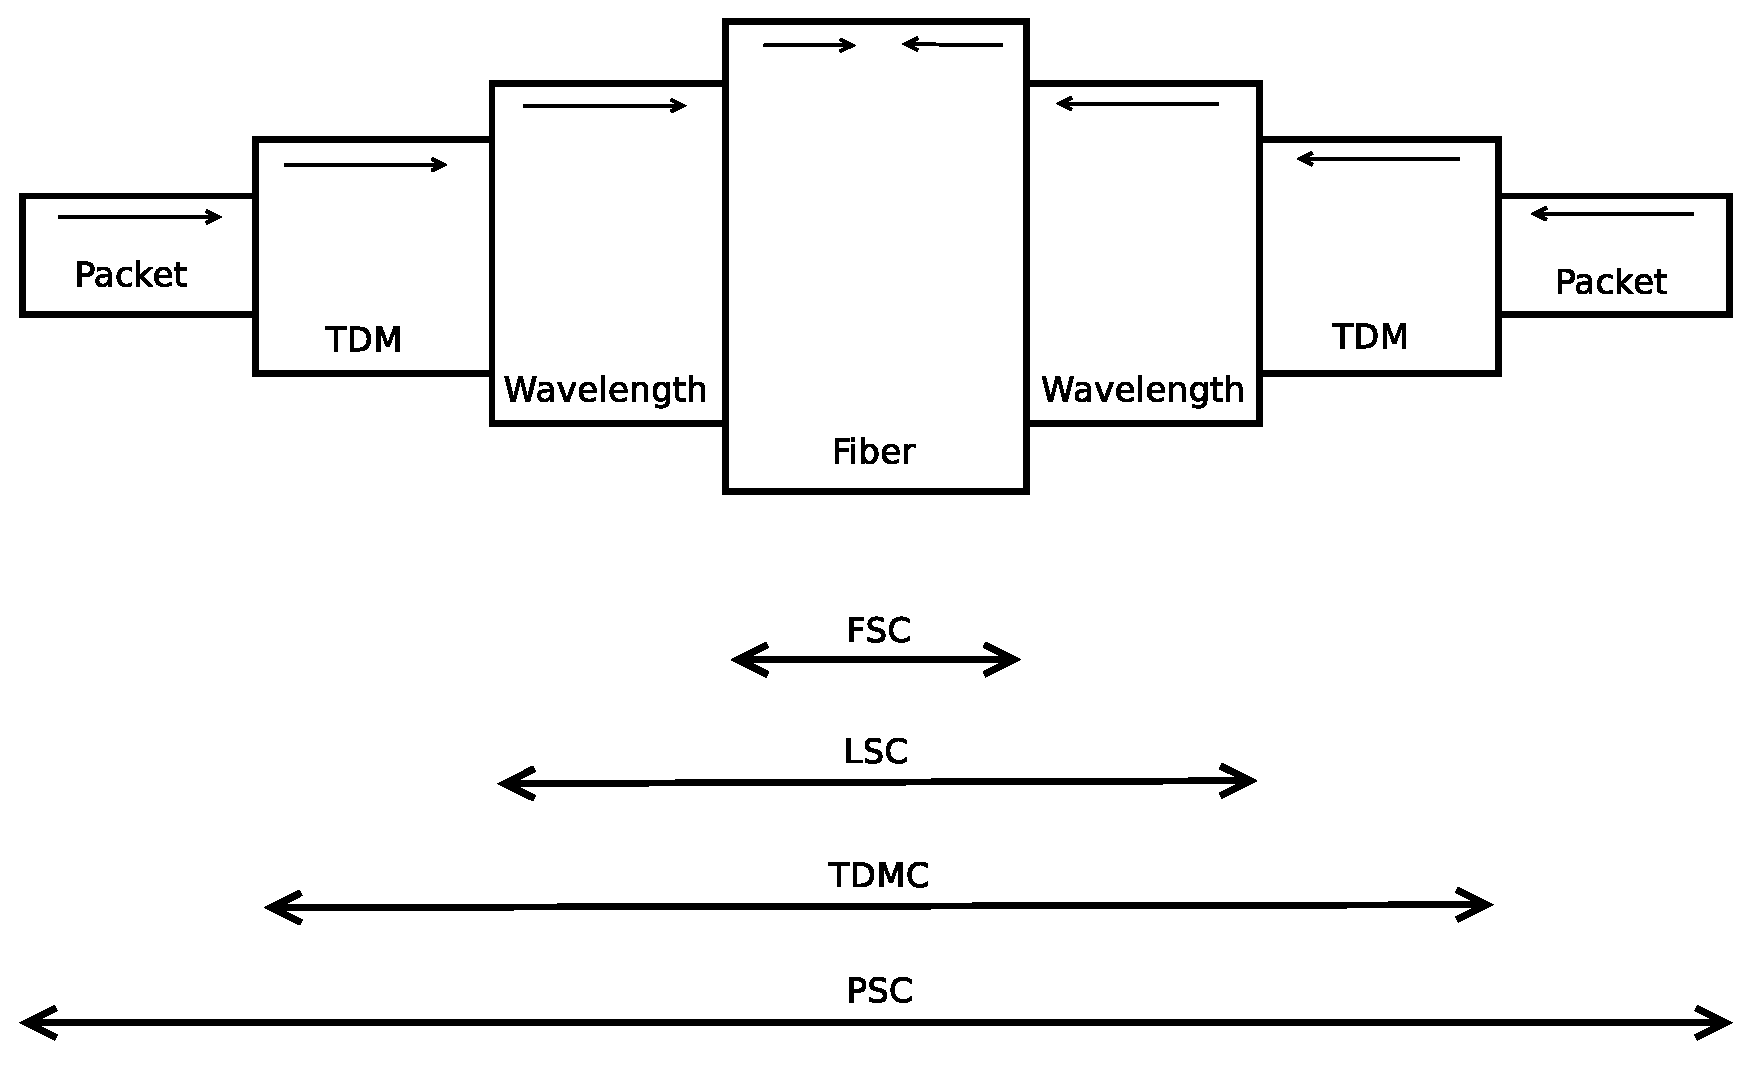
\includegraphics[width=0.9\textwidth]{img/gmpls_hierarchy}
  \end{figure}
}
\frame
{
  \frametitle{An example of a multi-layer path}

  \begin{figure}[!htbp]
    \begin{center}
      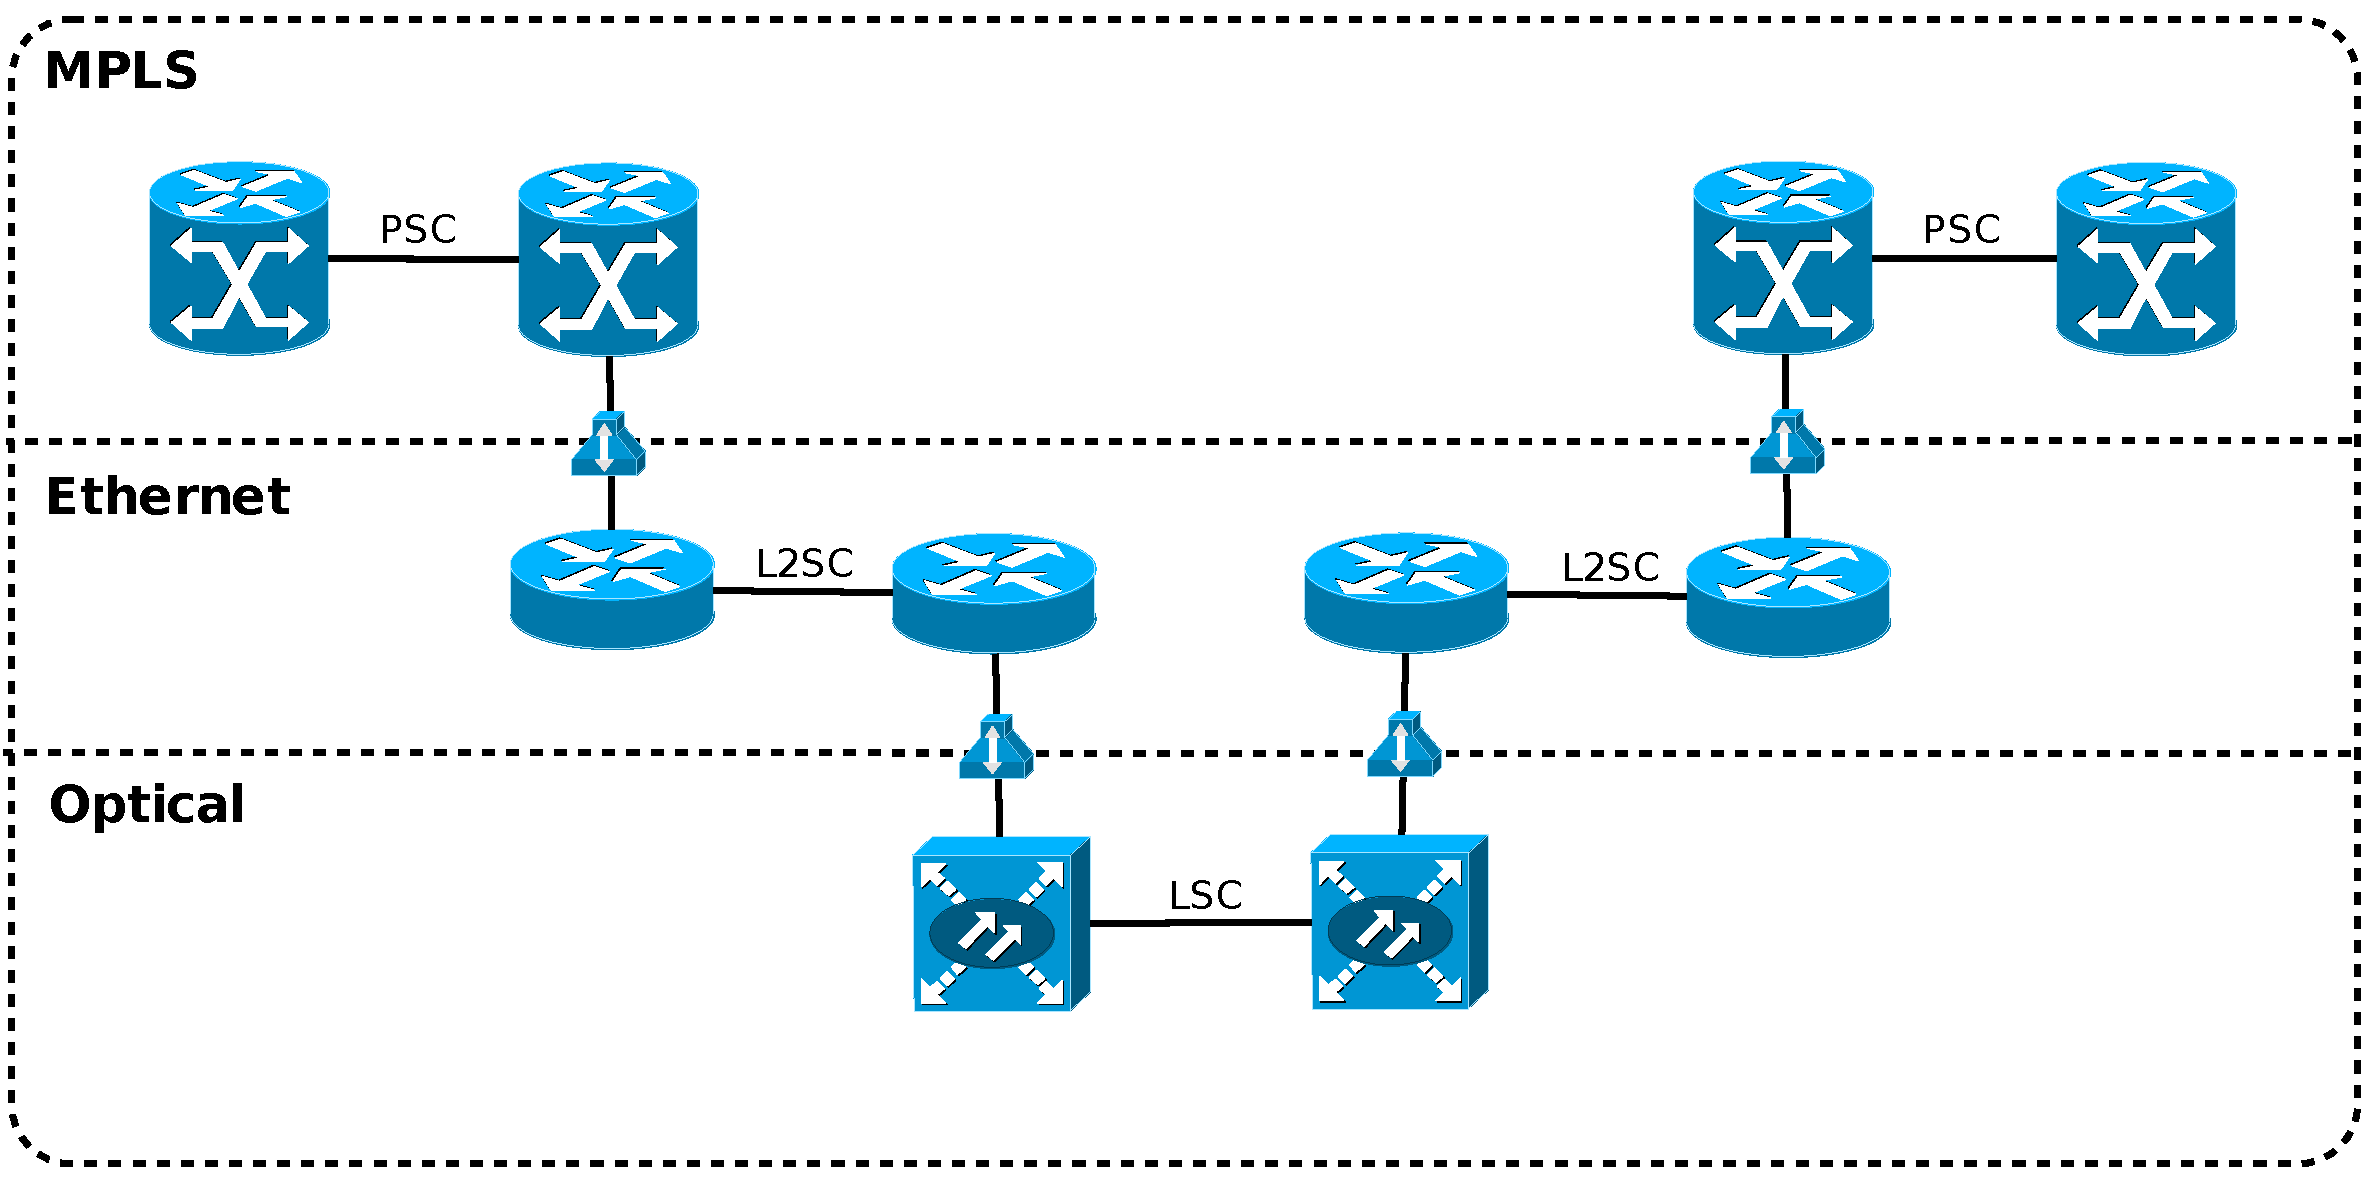
\includegraphics[width=1\textwidth]{img/multi_path}
    \end{center}
  \end{figure}
}
\frame
{
  \frametitle{GMPLS protocols}
  
  The most important protocols extended in GMPLS are:
  \begin{itemize}
  \item \textit{routing protocols}, which manage information about the
    network topology, i.e.\ IS-IS and OSPF-TE.
  \item \textit{signaling protocols}, which manage the reservation of
    network resources and guarantee a certain QoS, i.e.\ CR-LDP and
    RSVP-TE.
  \item \textit{link management protocols}, like LMP, which task is to
    discover and verify the connectivity of the links. 
  \end{itemize}
}

\section{Software Implementation}
\subsection{The DRAGON suite}
\frame 
{ 
  \frametitle{The DRAGON suite}

  The Dynamic Resource Allocation via GMPLS Optical Networks
  (\textbf{DRAGON}) software suite is a open source GMPLS suite, which
  goal is to prove the power and the flexibility of multi-layer
  networks in order to enable dynamic end-to-end service provisioning.

}
\frame
{
  \frametitle{DRAGON architecture}

  \begin{figure}[!htbp]
    \begin{center}
      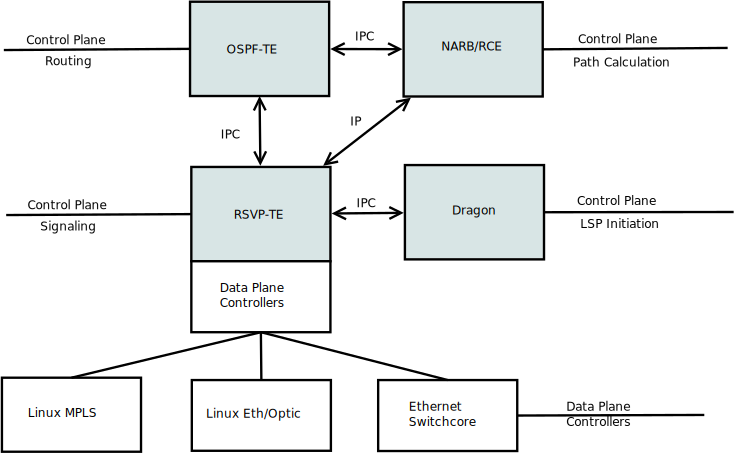
\includegraphics[width=0.9\textwidth]{img/dragon_model}
      \label{fig:dragon_model}
    \end{center}
  \end{figure}
}
\frame
{
  \frametitle{RCE architecture}

  \begin{figure}[!htbp]
    \begin{center}
      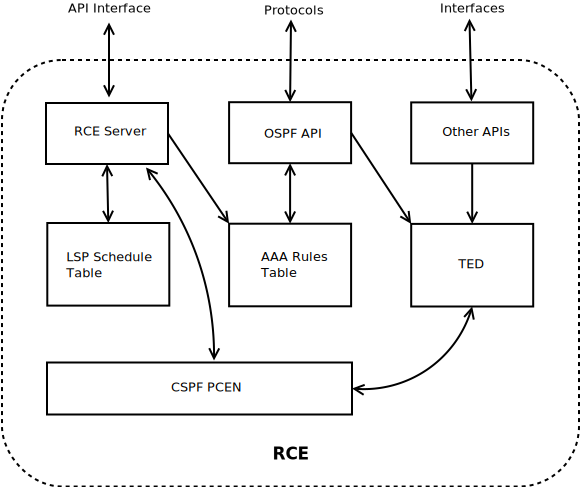
\includegraphics[width=0.65\textwidth]{img/rce_model}
    \end{center}
  \end{figure}
}
\frame
{
  \frametitle{PCEN Module}
  
  \begin{figure}[!htbp]
    \begin{center}
      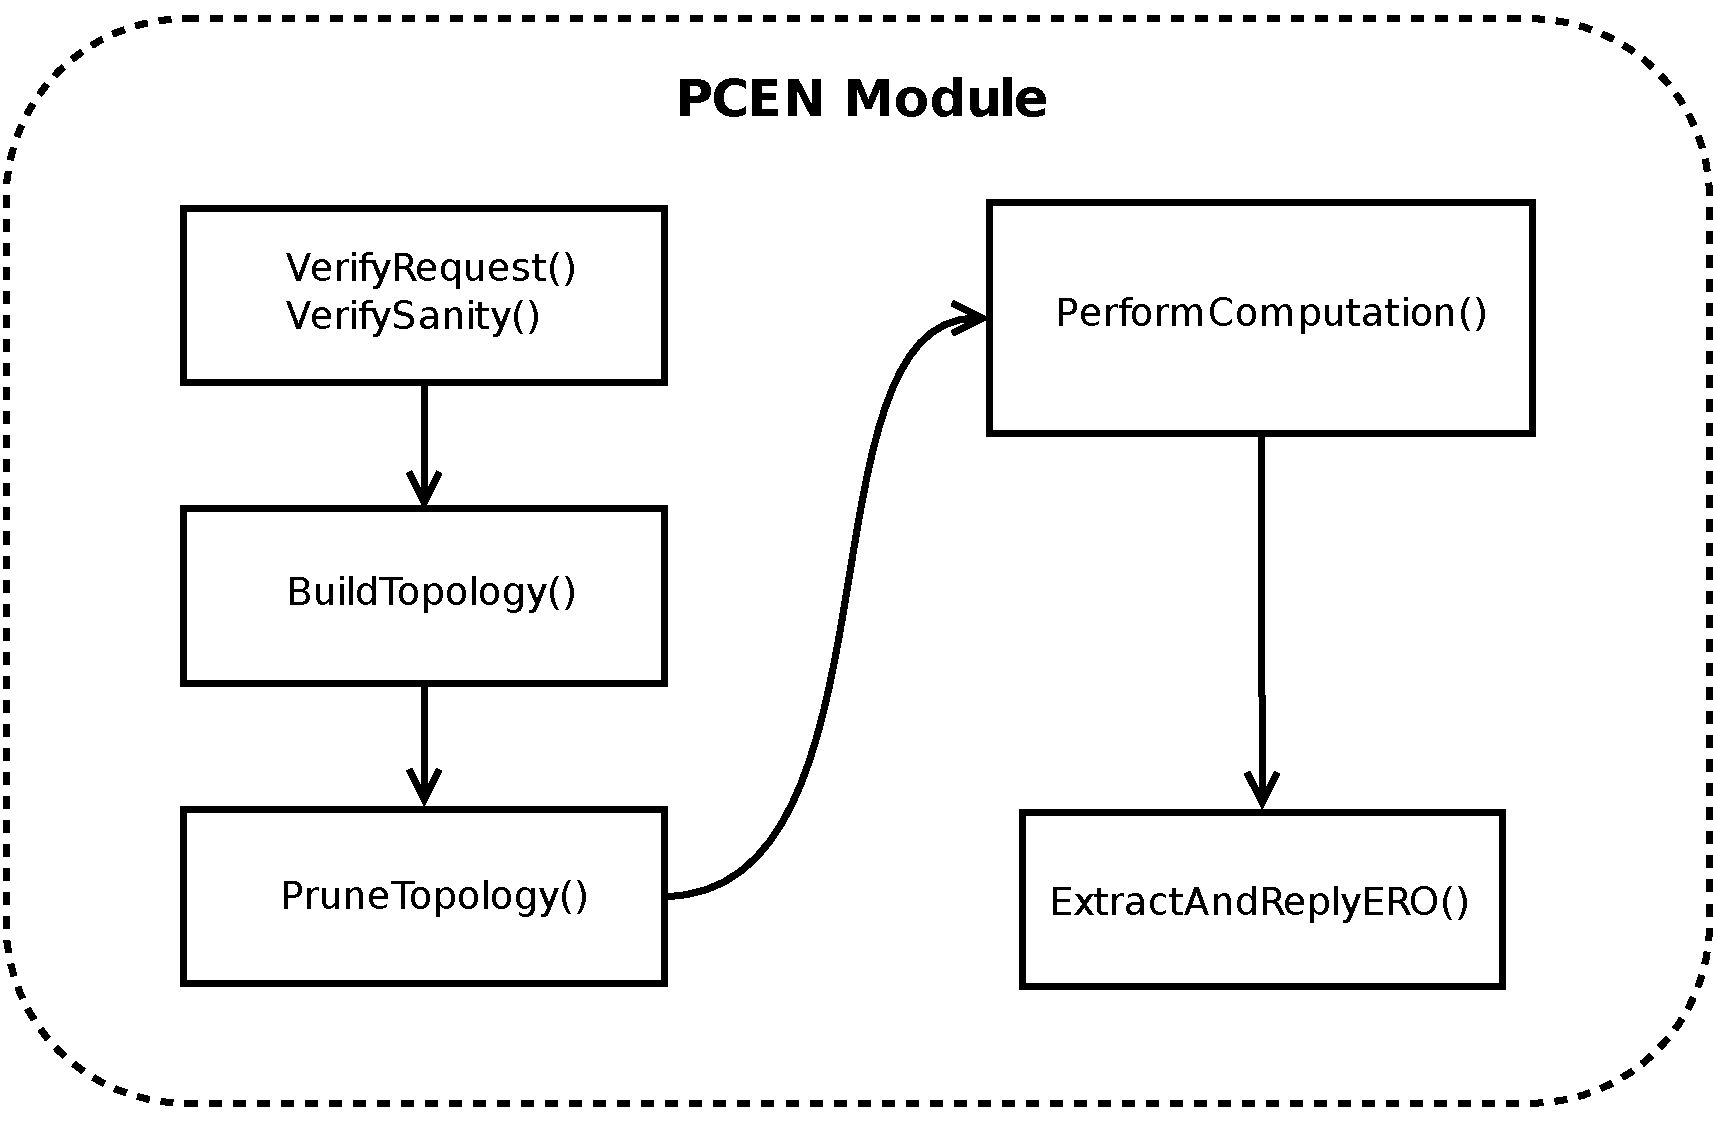
\includegraphics[width=0.8\textwidth]{img/pcen_module}
    \end{center}
  \end{figure}
}
\frame
{
  \frametitle{Candidate CSPF Algorithm}

  \begin{itemize}
  \item<1-> The implemented CSPF algorithm is derived from the BFS
    algorithm and searches for the loop-less paths between a source
    and a destination inside a multi-layer network.
  \item<2-> The constraints considered include general constraints,
    like bandwidth or accumulated metric, or layer-specific
    constraints, like wavelength continuity in the optical layer.
  \item<3-> A set of user-defined constraints has been supported to
    offer a better level of customization and flexibility.
  \end{itemize}
}
\frame
{
  \frametitle{Performance evaluation}

  Different test-cases have been considered: 

  \begin{figure}[!htbp]
    \begin{center}
      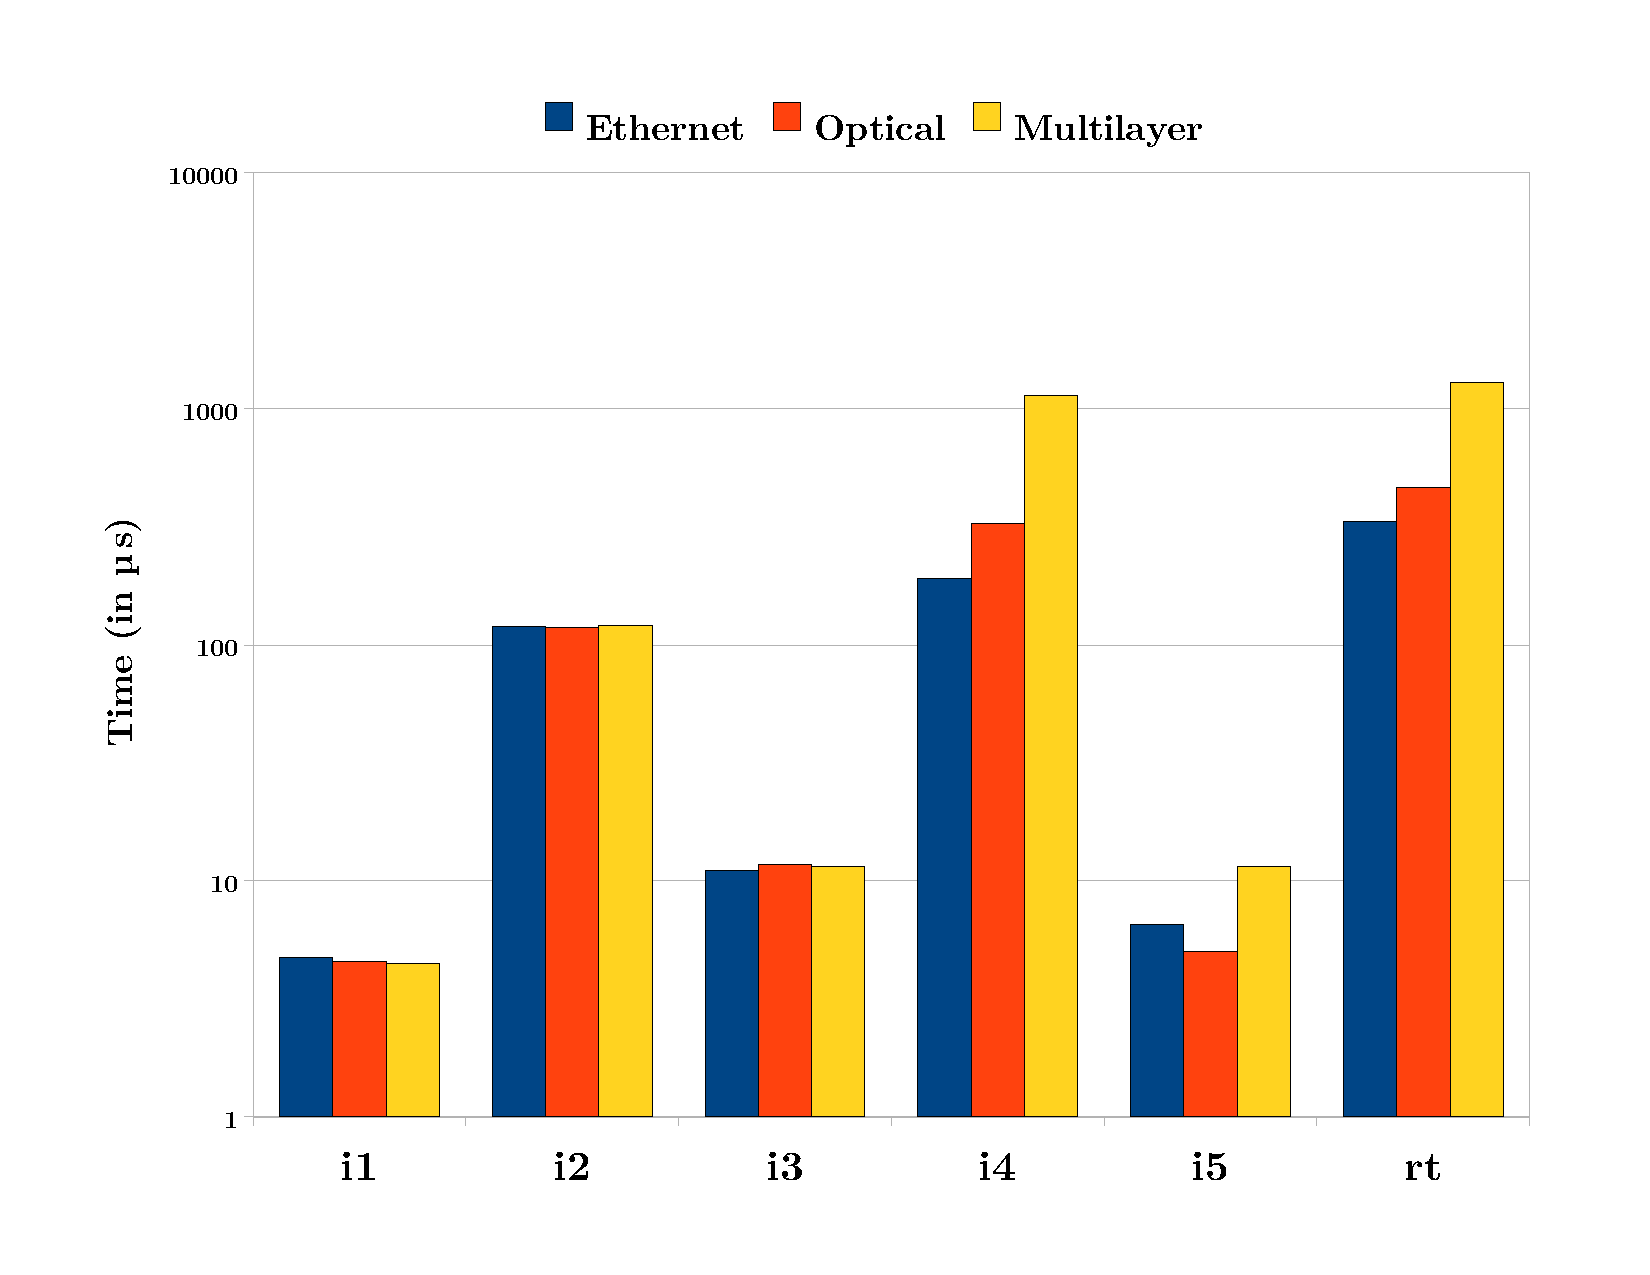
\includegraphics[width=0.72\textwidth]{img/time_graph}
    \end{center}
  \end{figure}

}

\section{Conclusions}
\frame
{
  \frametitle{Conclusions}

  This thesis work have been focused on the improvement of the
  automatic path-setup process in a complex multi-layered network:

  \begin{itemize}
  \item<1-> A path computation algorithm has been developed and thoroughly tested,
    proving that it is feasible to simplify the current manual process
    with a faster and more dynamic one. 
  \item<2-> The implemented solution can handle successfully a wide
    range of path constraints, showing also the capability of adapting
    itself in case of network topology changes; in addition, the support
    of user-defined constraints makes the system more flexible, allowing
    a finer degree of configuration.
  \end{itemize}
}
\frame
{
  \frametitle{The End}

  \begin{center}
  Questions?
  \end{center}
}

\end{document}

%%% Local Variables: 
%%% mode: latex
%%% TeX-master: t
%%% compile-command: "latexmk -pdf ju_liu_presentation"
%%% Local IspellDict: english
%%% End: 
